\documentclass[a4paper,11pt]{article}
\usepackage[utf8]{inputenc}
\usepackage[english]{babel}
\usepackage[a4paper]{geometry}
\usepackage{graphicx}
\usepackage{epsfig}

%opening
\title{Domain analysis: Integration of verification tools}
\author{Jeroen Kleijn}

\begin{document}

\maketitle

\section{Rationale}

Advances in chip technology have led to increasingly more and more complex chip
architectures. This raise in complexity has forced researchers in the field of
modern chip architecture to search for techniques which allow them to better cope
with this complexity. One of these techniques is xMAS\cite{chatterjee10,xmas}, a visual modeling
language that allows the description of system-on-chip designs using high-level constructs.

The WickedXmas\cite{13_toolxmas} tool was created to support the design of these network
models. Initially this tool primarily allowed visual diagramming of xMAS networks.
Over time, the tool has been extended with verification tools that allow static
analysis of the designs.

Like many other software projects, the WickedXmas tool has suffered from a decay in
software quality due to continuous modifications and the addition of new features.
Integration of the design part of the tool and the verification tools is suboptimal.
Using the verification tools is a cumbersome process for the end user requiring many
steps to perform. Furthermore, from a software architecture point of view, the tool
is hard to maintain and extend. Many dependencies on external libraries and utilities
severely hamper portability and deployability of the software.

In order to solve above mentioned issues, a complete rewrite of the WickedXmas tool is
warranted. Work has already been started on refactoring the available verification tools.
One of the key design issues involves the extensibility of the software. It should be
easy to code and integrate new verification tools. In addition, the design tool and
the various verification tools should integrate well.
To achieve this level of integration the source code of the new verification tools has
been examined as part of this domain analysis. The remainder of this document will describe
the structure of the source code and provide suggestions how the desired level of integration
can be reached.

\paragraph{Note:}
One of the assumptions made during this analysis is that the final design tool will be
written in c++. This assumption allows to investigate the ways in which the data structures
used by the verification tools can be shared with the design tool. Although this assumption
is likely valid, results from other domain analyses might express a preference for an
other choice of programming language.

\tableofcontents

\newpage

\section{The WickedXmas tool}


Before exploring the internals of the source code we shall first provide an overview
of the current WickedXmas tool. Specifically, we will briefly highlight the steps involved in
executing the verification modules.

\begin{figure}[h]
  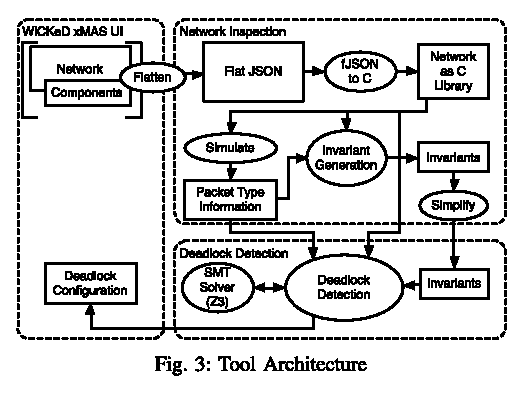
\includegraphics[height=5cm]{wickedxmas-arch.eps}
  \caption{WickedXmas Tool Architecture}
  \label{fig:wickedxmas-arch}
\end{figure}

Figure \ref{fig:wickedxmas-arch}\cite[p.~3]{13_toolxmas} depicts the WickedXmas tool architecture.
The design tool (WiCKeD xMAS UI) stores the network in a text file using JSON notation. Before
presenting the network to the verification modules (Network Inspection and Deadlock Detection),
the network description is flattened. This process transforms the hierarchical network into
a flat list consisting solely of xMAS primitives and the channels connecting their ports. The resulting
flat json file is then parsed and transformed into C++ source code. The generated source code files are
used along with C++ code written for the specific task to create several executables. In Figure
\ref{fig:wickedxmas-arch} the Simulate, Invariant Generation and Deadlock Detection verification modules
are shown. The executables must be run in a fixed order; results from a module can serve as input for modules further down
the pipeline. For instance, the Simulator runs a simulation on the network and yields information on the
types of packets each component in the network is able to accept and generate. The Invariant Generation
uses this information to deduce invariants that hold for the given network. Finally, the Deadlock Detection
module uses both the Packet Type Information and (simplified) Invariants to perform its task and present
the results back to the xMAS UI.

\paragraph{Dependencies}
Several utilities are used while performing these tasks. The conversion from JSON to C++ code is
handled by a javascript file and processed by phantomjs. A Haskell program takes care of the
Invariant simplification task. To compile the C++ code and link the object files to form the
executables a C++ compiler is required. The use of all these different utilities reduces the
deployability of the WickedXmas tool. All utilities must first be installed on the target system used
to run the tool.

\newpage

\section{New verification modules}

\paragraph{}
In order to improve the software quality the verification modules are currently being refactored.
Central to this process is the use of a single set of data structures used by all verification modules.
All modules are (or will be) written in C++ (C++ 2011). While designing the new data structures
special attention has been paid to ensure extensibilty. The data structures should not only be
able to provide current needs but also allow the integration of new verification modules. As of this
writing, several modules have been ported to use the new data structures in varying degrees. One
module that has been completely ported is the Combinatoric Cycle Checker. We will use this module
as an example to illustrate the use of the data structures. This module is relatively easy to
understand and will therefore serve us well as an example.

\subsection{xMAS data structures}


\begin{figure}[h]
 \includegraphics[width=\textwidth]{images/xmas-components}
 \caption{xMAS Class Diagram}
 \label{fig:xmas-components}
\end{figure}

\paragraph{}
In this section we will explore the new data structures. Figure \ref{fig:xmas-components} shows a
UML-diagram describing the core xMAS data structures. Each component in an xMAS network is represented
by an instance of the abstract XMASComponent class. All components can be identified by their unique name.
A component has an arbitrary number of ports, the number and type of ports depends on the actual
component type. For the currently defined primitives, this number varies between 1 and 3.\\
A port is represented by the Port class. Like XMASComponent, this class is an abstract base class. Actual instances
of Port are either an Input or an Output. Ports are identified by their name just like components.
Usually, ports have short identifiers like ``a'' and ``b''. 
\paragraph{}
The channels of an xMAS network have no direct class equivalent in the data structures. Rather, a channel is
formed by the connect() function. Input and Output both contain a pointer to an object of the opposite type.
The connect() function takes an Input and Output and updates these pointers such that they mutually
reference each other. The values of these pointers are guarded by an important invariant. At all times, 
except of course during connect(), an Input should either be disconnected or point to an Output which
in its turn should point back to the Input. The same statement should hold when switching the roles of
Input and Output.

\paragraph{}
Looking at the operations defined on Port, we can divide them into several categories.
\begin{itemize}
 \item The first category of operations deals with the identity and status of the port
 \begin{itemize}
  \item The Port constructor, destructor, getComponent() and getName() are self-explanatory. They initialize,
  destroy and query the attributes of a Port.
  \item isConnected() returns whether the port is connected to an other port or not.
  \item isConnectedTo(XMASComponent) returns whether this port is connected to a port of the specified component  
  \item valid() checks if the port is connected and, additionally, if the invariant mentioned earlier holds
  for this port.
 \end{itemize}
 
 \item The second category of operations provide information on the channel formed by this port
 \begin{itemize}
  \item connect() has been explained above, this operation establishes a channel between two ports
  \item getTarget() and getTargetPort() return the component and its port that are on the receiving end
  of the channel. The target port thus is an Input to the component returned by getTarget().
  \item getInitiator() and getInitiatorPort() return the component and its port that are on the sending end
  of the channel. The target port thus is an Output from the component returned by getInitiator().
 \end{itemize}
  The presence of these methods show the dual role of class Port. It represents not only a port in an
  xMAS network, but also the channel between two ports, of course provided the port is actually connected.
  The channel-role is equally well fulfilled by either port.
 \item The other operations: accept, getPortExtension and clearPortExtension will be explained in detail
 in the next sections.
\end{itemize}

\paragraph{}
Returning our focus to XMASComponent we notice many operations similar to those of Port.
\begin{itemize}
 \item The constructor and getName() operations set and query the name of the component.
 \item valid() returns true if all ports of the component are valid and false if at least one port is not valid.
 \item beginPort() and endPort() return iterators to loop through all available ports. The type arguments
 can be used to specify if only input, output or all ports should be returned.
 \item accept and the -Extension functions will be covered in the next sections.
\end{itemize}

XMASComponent itself is an abstract class. Each of the 8 xMAS primitive types is represented
as a separate class inheriting from the XMASComponent base class. Whereas XMASComponent only provides
access to ports, the primitive classes actually instantiate them. Some primitive types have additional
attributes, e.g. XMASQueue has an attribute to indicate the queue capacity. Maybe surprising is the 
fact that other primitive types seem to lack the required extra attributes. For example, XMASFunction
has no attribute to hold the function to apply to the data packets and XMASSource has no attribute
specifying what type of packets it should produce. These seemingly missing attributes are stored using
the extension mechanism covered in the next section.



\subsection{Extensions}

\paragraph{}
The classes that represent the 8 xMAS primitives and their base class XMASComponent provide few features
to support the verification modules. For instance, many modules need to know what packet types a component can
accept or produce but neither XMASComponent nor its descendants are able to provide this information.
This design is a deliberate choice. The classes only expose core attributes like their name and the
ports that are available. However, all components allow extra data to be stored in so called extensions.
The same mechanism is available to augment ports with arbitrary extra data.

\begin{figure}[h]
 \includegraphics[width=\textwidth]{images/xmas-hierarchy}
 \caption{xMAS Class Hierarchy}
 \label{fig:xmas-hierarchy}
\end{figure}

\paragraph{}
Figure \ref{fig:xmas-hierarchy} shows the classes that implement the extension mechanism. Both XMASComponent and Port are
actually part of a relatively complex class hierarchy.
At first sight, the extension mechanism appears to be quite complicated. The basic idea, however, is
very simple. All ports are able to hold a list of PortExtension objects, likewise,
all components are able to hold a list of XMASComponentExtension objects. Any module can define a new
Extension class (e.g. CombinatorialCyclePortExtension) and make it a subclass of either PortExtension
or XMASComponentExtension, depending on whether the extension stores attributes of a port or of a component. 
The ExtensionContainer class provides methods to add, remove and fetch the extensions of a given type.
For instance, the cycle checker will call getExtension() using CombinatorialCyclePortExtension as
the template parameter T.

\paragraph{}
The linked list of extensions could easily have been implemented using the default STL container
classes, like std::list or std::forward\_list. The chosen design has a few important advantages.
The first one is related to the pointers required to maintain the list. Here, each extension
stores the pointer inside the extension itself by inheriting the next attribute from Extension.
This approach, called internal storage\cite{linkedlist}, differs from the approach used by the STL lists.
External storage, as used by STL, is the more generic approach as it places no constraints on
the value type (see \cite{linkedlist} for details). Since the data structures are self-developed
and can be designed to incorporate internal storage, the space and run time performance benefits
of internal storage outweigh the extra effort.

\paragraph{}
The second aspect of the extensions design concerns type checking. In the diagram this aspect
is reflected through the use of the generic Extension class and its type attribute. The main
benefit of this design decision is again performance but additionally it improves type safety.\\
Each component (or port) holds a heterogeneous list of extensions, each derived from XMASComponentExtension
(or PortExtension for ports). By equipping class Extension with a template parameter the next attribute's
type can be accurately specified. To illustrate this, let's take a look at the definition of PortExtension:\\\\
\emph{class PortExtension : public Extension\textless PortExtension\textgreater \textbraceleft \\
\textbraceright}\\\\
The template parameter E of Extension is bound to PortExtension. The result is that the next attribute
that PortExtension inherits from Extension has type PortExtension*. The compiler can now check that the
list actually contains extensions derived from PortExtension.

\paragraph{}
Although the linked list is guaranteed to only contain valid extension types, most verification
modules are only interested in specific subclasses of PortExtension or XMASComponentExtension.
ExtensionContainer provides methods to efficiently filter the list of extensions.
getExtension\textless T\textgreater () returns the first extension whose type matches that of
template parameter T. getExtensionOfBaseType\textless T\textgreater () also select extensions
that are derived from T. The type attribute defined in Extension aids ExtensionContainer to
select the correct Extension.\\


\subsection{Visitor Pattern}

\paragraph{}
The extension mechanism enables verification modules to augment components and ports with
arbitrary extra data. Many times it is desirable to extend the behavioural features of the
classes as well. The Visitor Pattern provides this behavioural complement to extensions.

\paragraph{}
When the Visitor Pattern is applied to an object-oriented class design, operations normally
defined on the domain classes are pulled out of the class and accomodated in a new class
known as a visitor. The Gang of Four defines the Visitor as:\\"Represent an operation to be
performed on elements of an object structure. Visitor lets you define a new operation without
changing the classes of the elements on which it operates."\cite{wiki-visitor-pattern}\\
The visitor pattern is essential for the modularity and extensibility of the verification
modules. Rather than implementing all verification code inside the domain classes, each
module defines one or more Visitor classes. Inside these classes the implementation of
the verification code is placed. Adding a new module does not require a single change to
XMASComponent, Port or any of the other domain classes.

\paragraph{}
The Visitor Pattern applied in C++ makes use of two features of the language. The first one
is function overloading. Overloaded functions have multiple distinct implementations while
all share the same function name. The functions however differ in the number and type
of arguments they operate on. When a compiler encounters a call to an overloaded function,
it inspects the arguments it should pass and uses this information to resolve the correct
function to call.\\
The second language feature is dynamic dispatch. Through the use of virtual functions the
actual function to invoke is determined at run time.\\
When used together, these features implement double dispatch. Overloaded functions allow
differentiation based on the arguments of the function, virtual functions allow differentiation
based on the actual type of the calling object.
\nocite{stroustrup}

\paragraph{}
In the class diagram two Visitor interfaces are defined, one for ports and one for components.
Visitors that implement interface PortVisitor must provide two implementation of the overloaded
function visit(). One to handle visits to an Input port and one to handle a visit to an Output port.
Likewise, implementations of interface XMASComponentVisitor must implement the visit method
for each of the 8 xMAS primitive types.

\begin{figure}[h]
 \includegraphics[width=\textwidth]{images/visitor-sequence-diagram}
 \caption{Visitor Sequence Diagram}
 \label{fig:visitor-sequence-diagram}
\end{figure}

\paragraph{}
Figure \ref{fig:visitor-sequence-diagram} shows the Visitor Pattern in action.
CombinatorialCycleDependencies is an implementation of the XMASComponentVisitor interface.
In this example, an instance of this class calls the accept method on an XMASComponent
instance, in this case an XMASMerge. Through dynamic dispatch the accept method as
defined by XMASMerge is called. The implementation of this method is:\\
\begin{verbatim}
void accept(XMASComponentVisitor &v) {
  v.visit(this);
}
\end{verbatim}

Immediately, control is returned to the Visitor class by calling its visit method. Since the method
is defined as part of the XMASMerge class, the this pointer passed has type XMASMerge*. The compiler
uses this knowledge to infer that it has to call the overloaded visit method which takes a pointer
to an XMASMerge component (overloading and dynamic dispatch are combined here to perform double
dispatch). The CombinatorialCycleDependencies class is now able to execute code specifically written
to handle an XMAS merge. The diagrams also shows a slightly more complex example where the Visitor
recursively calls accept on an XMASQueue instance during the processing of a visit to an XMASFork object.


\paragraph{Open/Closed Principle}
Both the Extension mechanism and the Visitor Pattern are applications of the Open/Closed
Principle. This principle states that: ``Software entities like classes, modules and functions
should be open for extension but closed for modifications''\cite{oodesign-open-close}. Minimizing
changes to existing classes that have been tested and used, prevents undesired effects
on current functionality. Core classes like XMASComponent and Port are used in many different parts
of the software (see also \ref{fig:xmas-headers}), so changes to these classes have impact on the entire application.
At the same time, the priniciple dictates that new features can still be added to the software entities.


\section{Combinatoric Cycle Checker}

\paragraph{}
The semantics of an xMAS network can be expressed using the concepts of a combinatorial part and
a sequential part\cite{analyse-tool-11}. The primitives can be divided into two categories.
Sources, sinkes and queues are known as sequential primitives. The other five: function,
fork, join, switch and merge are combinatorial primitives.\\
Each clock tick a source can produce a packet, a sink can consume one and a queue can accept
and/or release a packet; all as long as the necessary conditions hold. The clock ensures
all sequential primitives are updated at the same time.\\
The combinatorial objects' task is to route the packets from one sequential primitive to another.
Of course, the time required to perform this routing depends on the amount and types of
combinatorial objects along the path from source to destination. But, as far as the simulation of
the network is concerned, the entire routing occurs during a single clock cycle.\\

\paragraph{}
One important aspect of an xMAS design is the absence of combinatoric cycles. That is, an xMAS
network should not contain cycles in the graph consisting of only combinatorial objects.
Would this be the case, the irdy and trdy signals of the combinatorial objects will never
stabilize. This can be seen by looking at the equations that define the irdy and trdy signals
\cite{chatterjee10}. The source and sink primitives irdy and trdy signals are determined by an
oracle (neglecting the \emph{pre} part for simplicity). Queues are defined to always accept
data (i.trdy = 1) as long as the queue is not full and release data (o.irdy = 1) as long as
the queue is not empty. All of these conditions, the oracles and the queue state, are well-defined
and independent of other components in the network.\\
In contrast, all combinatorial objects' irdy and trdy equations are defined in terms of the
irdy and trdy signals produced by the components on the other sides of the channels.
To determine an irdy or trdy signal of a combinatorial primitive, the connected components'
irdy and trdy signals should be substituted in the equation. Large chains of combinatorial
primitives as such yield complex expressions. More so, when a component is part of a
combinatorial cycle, the state of the irdy or trdy signal occurs on both the left-hand and the right-
hand side of the equation. Substitution of the right-hand side occurrence of the signal leads
to an infinite recursion.

\begin{figure}[hp]
 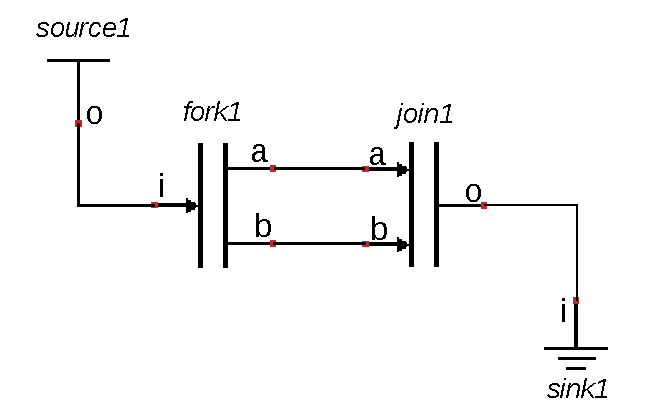
\includegraphics[height=3cm]{images/fork-join-cycle}
 \caption{Example of a combinatorial cycle}
 \label{fig:fork-join-cycle}
\end{figure}

\paragraph{Example}
Figure \ref{fig:fork-join-cycle} illustrates a combinatorial cycle. Applying the \emph{a.irdy} equation
to \emph{fork1} and the \emph{b.trdy} equation to \emph{join1} gives \cite[p.~44]{chatterjee10}:
\begin{itemize}
 \item fork1.a.irdy := fork1.i.irdy and fork1.b.trdy = source1.o.irdy and join1.b.trdy
 \item join1.b.trdy := join1.o.trdy and join1.a.irdy = sink1.o.trdy and fork1.a.irdy
\end{itemize}
Substituting the second equation in the first now gives:
\begin{itemize}
 \item \underline{fork1.a.irdy} := source1.o.irdy and sink1.o.trdy and \underline{fork1.a.irdy}
\end{itemize}







\paragraph{The Combinatoric Cycle Checker}
The Combinatoric Cycle Checkers job is to detect these combinatorial cycles in an xMAS network.
It is based on a standard graph traversal algorithm to detect cycles. For all ports of all
components in the model, the algorithm executes a depth-first traversal. At each step, the
traversal continues according to the signals on the right-hand side of the equations
of the current component. For input ports this equation is the one that defines
the trdy signal, for output ports this equation is the one that defines the irdy signal.\\
Along the traversed path, each port, including the starting port, is marked as 'checking'.
If the algorithm later visits this port again, it knows it has detected a cycle.
The traversal along a path ends when it reaches a sequential component. During backtracking,
all 'checking' marks are reset. If none of the paths starting from a port result in a
combinatorial cycle, the port will be marked as 'checked'. The Cycle Checker has completed
when all ports have been marked as 'checked'.





\paragraph{Implementation}
The Combinatoric Cycle Checker is implemented using an extension class, a component visitor
and several functions to drive the checker. Class CombinatorialCyclePortExtension is, as
the name already suggests, a PortExtension. It holds two boolean attributes: \emph{checking} to
indicate whether the algorithm is currently traversing this port and \emph{checked} which is
set to true after the port has been successfully checked.\\
CombinatorialCycleDependencies is an implementation of the XMASComponentVisitor interface.
The constructor takes a pointer to the Port object that was used to reach the component
currently being visited. Attribute \emph{p} is initialized with this value. A second attribute,
\emph{retval}, is an initially empty vector of ports. The various visit member functions will
fill this vector with the ports that the algorithm should use to continue the traversal. Visits
to the sequential primitives will leave this vector empty. When a combinatorial primitive is
visited, all ports required to evaluate the irdy or trdy signal of \emph{p} are added to the vector.

\paragraph{}
Inside function checkSignal() the actual algorithm is executed. It is here where the PortExtension
is created and the \emph{checking} and \emph{checked} values are set. Also the visitor class
is instantiated and used to visit the component. Depending on the contents of attribute
\emph{retval}, the algorithm recursively continues its traversal. The Cycle Checker is started
by calling CombinatorialCycleDetector and passing the set of all components.

\newpage

\section{Integration of Verification Tools}

\paragraph{}
Ultimately, the verification tools must be integrated with the new WickedXMas design tool.
This section provides suggestions how to realize this integration.

\subsection{Tool Architecture}
\label{sec:tool-architecture}

\paragraph{}
In the WickedXMas Tool Architecture the design tool and the verification tools
are clearly separated software components. The tools are written in varying languages
and they are implemented as separate executables. Now that all tools are being rewritten
in a common language (C++), more efficient communication between the verification tools
is possible. All tools are integrated into a single executable which is executed as a
single process. Due to this, the tools share the same address space and can directly
access information produced by other tools.\\

\paragraph{}
With regards to the integration with the design tool, two choices are available.
\begin{enumerate}
 \item The design tool could be integrated completely with the verification module.
 \emph{(in-process)}
 \begin{itemize}
  \item Not only the verification tools but also the design tool become part of a single
  application. Both the design tool and the verification modules operate on the same
  copy of the xMAS data structures.
 \end{itemize}

 \item The design tool and the verification tools are implemented as two separate
 programs. \emph{(out-of-process)}
 \begin{itemize}
  \item The design tool launches the verification tools as a new process. Inter-process
  communication mechanisms are used for communication between the two programs.
  \item Both software components have their own representation of an xMAS network. The
  design tool can not directly access the data structures of the verification tools.
  However, the design tool can reuse source code, like the classes used by the verification
  tools (XMASComponent, Port, etc.). (See also section~\ref{sec:extensions-visitor-design-tool})
 \end{itemize}
 
\end{enumerate}



\subsection{Module dependencies}

The execution time of the modules can vary greatly. When large networks are provided as input to the
modules, algorithms with high run time and space complexity may consume many system resources. Therefore,
it might be desirable to disable some verification modules if their results are currently not of interest.\\
The xMAS data structures have been designed with modularity and independency in mind. But, as shown in
the WickedXMas Tool Architecture, the verification modules don't operate in a completely isolated
fashion.\\
The order in which the modules are executed is important. Some module can only be executed after
the results from other modules are available. In order to provide flexibility in the choice of
verification modules to run, careful design of the verification modules is necessary.
If possible, the most time consuming algorithms should be easy to disable. That is, other modules
should minimize dependency on the results of those modules.


\subsection{Using Extensions and Visitors for the design tool}
\label{sec:extensions-visitor-design-tool}

\paragraph{}
The use of Extensions and Visitors is not limited to just the verification modules.
The same mechanisms can be utilized by the design tool. Properties like the
position and orientation of an xMAS component on the design canvas can be
stored in a new Extension class. The Visitor Pattern can be used for
tasks like rendering an image of a component on the canvas. Another use of
the pattern is to export xMAS networks to other representations like Verilog.

\paragraph{Composite objects}
There is however one issue that requires some thought. The verification modules
currently have no notion of composite objects. The design tool on the other hand
makes heavy use of composite objects to maintain a clear overview of the network.\\
We briefly explore three approaches to resolve this issue. All approaches assume that
a new class, XMASCompositeObject, is introduced to represent a composite object.

\paragraph{}
In the first approach the XMASComponentVisitor interface is extended with an
additional method to visit a composite object. The implementations of XMASComponentVisitor
use the methods of XMASCompositeObject to obtain access to the ports and components
inside the composite object. This approach is easy to implement. The downside is
that all verification modules have to be adjusted to implement the new XMASComponentVisitor
interface.

\paragraph{}
The second approach tries to hide the existence of composite objects altogether
from the verification modules. Rather than extending the Visitor interface,
the accept method of XMASCompositeObject is implemented in a non-default way.
Instead of passing itself as the argument to visit, the composite object calls
the accept method on all components inside the composite object, essentially
performing the flattening step.\\
The benefit of this approach is that it requires no changes to existing modules.
On the downside, this approach is harder to implement. Care has to be taken
that the transparency of composite objects is complete. For example, the objects
returned by the getInitiator() and getTarget() methods of Port must not return a
XMASCompositeObject object since the modules are likely to use these methods.
Possibly special CompositeInput and CompositeOutput classes are required in
order to implement this approach.\\
Another issue is that transparency is not always desirable.
Unlike the verification modules, the design tool sometimes prefers to
view a composite object in its entirety while at other times the design
tool wants to access the components inside the composite object.\\
Whether this second approach is feasible remains a question.

\paragraph{}
A third approach explicitly executes the flattening step. The design tool
uses a separate copy of the data structures. Before the network is
presented to the verification modules, all composite objects are flattened
to create a network without composite objects. Like the second approach,
existing verification modules need no modifications. Memory usage will
increase though to store the two different views of the network. Also,
feedback from the verification modules must be translated back to the
original network model with composite objects.




\subsection{Feedback from tools}

\paragraph{}
Feedback produced by the tools can be presented back to the design tool
in several ways. In this section, the types of feedback and possible
ways to present feedback to the design tool are covered.

\subsubsection{Types of feedback}
Verification modules may want to provide various types of feedback:
\begin{itemize}
 \item errors found in an xMAS design, for example
 \begin{itemize}
  \item a combinatoric cycle detected by the cycle checker, the design tool
  could highlight the components and channels that are part of the cycle.
  \item an error in a function specification
 \end{itemize}

 \item information which might be interesting to the user, for example:
 \begin{itemize}
  \item invariants
  \item packet type information
 \end{itemize}

 \item progress information
 \begin{itemize}
  \item Gives the user an indication of the remaining time required by a
  verification module to verify a network. Not all algorithms are able to
  provide an accurate progress indication.
 \end{itemize}


\end{itemize}


\subsubsection{Feedback communication}

\paragraph{Send feedback to an ostream}
Currently, the verification modules use the standard output stream (stdout)
to send feedback (and debugging information) to the user. By generalizing this
method to output feedback to an arbitrary ostream, this mechanism can also be
used to stream the feedback to the design tool. In order for the design
tool to interpret the feedback, a well defined data format must be agreed upon.
This format must be capable of transmitting all types of feedback. Also,
a convention to refer to entities like components and ports must be agreed upon.

 
\paragraph{Define a custom feedback streaming interface}
Instead of the (character based) ostream, the verification module passes feedback
through a streaming interface specifically written for this purpose. Possible
operations this interface might expose include:
\begin{itemize}
 \item info(XMASComponent* component, string message)
 \item error(Port* port, string message)
 \item progress(int progress, int total)
\end{itemize}
Multiple implementations of this interface can be written. For instance, one
implementation could simply write the feedback to stdout, using the same output
format as above. Another implementation could directly access the data structures
passed, e.g. the XMASComponent of the info operation in the example. In this case,
the design tool doesn't have to parse the character stream and lookup the component.
The design tool and the verification modules must share the same address space for
the latter implementation to work correctly though.


\paragraph{Let design tool read extensions defined by modules}
Unlike the previous methods, the verification modules don't send feedback to
the user at all. Rather, the design tool accesses the extensions created by the
verification  tools to gather information. When using this method, the feedback is
pulled by the design tool instead of pushed by the verification modules. As a result,
the verification modules need only expose their data through the extensions. The
design tool can decide what information it actually needs and fetch it by itself.
Detailed and tool-specific information can be communicated without the need to
define an interface capable of transmitting all message types.\\
Drawbacks of this method include the increased coupling between design tool and
verification modules. The design tool must know which extensions each verification
module uses and write custom code to extract and display the feedback. Another
issue is that information like progress is hard to extract from just the extensions.
If possible at all, this would require periodic polling of all components/ports in the
network to check their status with regards to a verification step.\\
Again, since the design tool directly accesses the extensions created by the verification
modules, the design tool and the verification modules must share the same address space.

\paragraph{Pass feedback to design tool by storing it in an Extension}
This method also uses the Extension mechanism to give the design tool access to the
verification tools' results. The difference is that all feedback is stored in
special Extension classes used purely for the purpose of passing feedback. The design
tool no longer needs to know about the internals of the verification tool, reducing
coupling. Like the previous method, detailed and tool-specific information is
available to the design tool, but this time, the verification modules must collect
the information and store it in the feedback extension.\\
The same issues with regards to progress information and the ``same address space``-
restriction apply.



\section{Recommendations}

Several options are available to integrate the design tool and the verification
modules. The recommendations in this section are based on two important use cases:
\begin{enumerate}
 \item the application will be used to design and verify xMAS networks
 \item the design tool will be used to develop and debug verification tools
\end{enumerate}

The use cases lead to different requirements. In order to support the first use case,
efficiency of the application is an important aspect. The design tool is an interactive
application and should be responsive. When verifying large networks, large amount of
memory and processing time can be consumed.\\
During development of the verification tools, efficiency is of less concern. Mainly
small networks are used to debug the tools. More important is the ability to support
an efficient 'edit-compile-run-debug' cycle. The source code of the verification
modules will frequently change. After a change has been made, the effort required to
test the new code should be kept at a minimum.

\paragraph{Tool Architecture}
Both architecture types discussed in section \ref{sec:tool-architecture}, in-process
and out-of-process, can be used to implement the two use cases. An in-process architecture
leads to more efficient communication between design tool and verification modules.
As such, the first use case would suggest to take this approach. As an additional
benefit, this approach is easier to implement.\\
However, an out-of-process might be better suited to support the second use case.
After a change has been made to a tool, only the source code related to the verification
tools has to be recompiled, reducing the time spent in the compile phase of the
'edit-compile-run-debug' cycle. Furthermore, the design tool doesn't even have to
be restarted to test the changes.\\
Another reason to opt for the out-of-process architecture is the ability to execute
the verification tools on an other, maybe more powerful, system.

\paragraph{}
Both architecture types have advantages and disadvantages. The relative importance
of the two use cases can be the decisive factor when choosing between them. Since
the intended use and target audience of the tool may change over time, it is
recommended to consider the possibility to change the architecture in the future.
Therefore, solutions that are only viable in both architecture types are preferred.


\paragraph{Communication}
Of the four communication methods described above, only the first two can easily be
used in an out-of-process architecture. The third and fourth both use extensions
and this requires either a shared address space between design and verification 
tools or an (platform specific) inter-process memory sharing technique. Although
the detailed information available in the extensions is an advantage of these methods,
simple text messages to describe the feedback are thought to provide enough information.
In most cases, the code required to 'push' feedback from the verification modules
is already in place which further reduces the advantages of the third method.

\paragraph{}
The first two methods are both good candidates. The second method has a few advantages,
especially when using an in-process architecture. Feedback can be passed more efficient,
due to the direct access to the components and ports. This is not very important though
as the feedback interface is very low traffic and data structures like hash maps allow
efficient lookup of the xMAS objects by id. However, since the second method is capable
of producing the same output as the first method and furthermore guarantees a consistent
data format output across all modules, the second method is recommended.

\paragraph{Composite objects}
The best way to deal with composite objects is not clear yet. Ideally, the verification
modules will be adapted to handle composite objects. This prevents any communication
issues that may arise due to the different network representations of the design tool
and verification modules. Modifying the verification modules might prove to be too
laborious. In this case, the network must first be flattened. Implicitly using the
second approach, or explicitly using the third approach.\\
The second approach is the technically more interesting approach and has the advantage
of a lower memory footprint. However, the simpler third approach is the safer option
and therefore recommended.


\paragraph{}
As a final note, if the design tool will be programmed in a language other than
C++, few options remain. Only an out-of-process architecture is possible. Code
written to create the verification modules can not be reused, although, of course,
the same classes and design patterns could be employed in most other languages.
The best option to establish the communication is through a character stream as
virtually all platforms and programming languages support this form of
communication.



\section{Glossary}
\begin{description}
 \item[(verification) module] 	Software component which applies a verification algorithm to an xMAS network
 \item[design tool]		Software component to visually model an xMAS network
 \item[Visitor class]		A software class that implements the Visitor interface
\end{description}

\begin{thebibliography}{9}

\bibitem{chatterjee10}
  Chatterjee, Kishinevsky, Ogras,
  \emph{Quick Formal Modeling of Communication Fabrics to Enable Verification},
  2010
  
\bibitem{xmas}
  Chatterjee, Kishinevsky, Ogras,
  \emph{xMAS: Quick Formal Modeling of Communication Fabrics to Enable Verification},
  2012
  
\bibitem{13_toolxmas}
  Joosten, Verbeek, Schmaltz,
  \emph{WickedXmas: Designing and Verifying on-chip Communication Fabrics},
  2012
  
  
\bibitem{linkedlist}
  \emph{https://en.wikipedia.org/wiki/Linked\_list\#Internal\_and\_external\_storage},
  november 2014
  
\bibitem{wiki-visitor-pattern}
  \emph{https://en.wikipedia.org/wiki/Visitor\_pattern},
  november 2014

\bibitem{oodesign-visitor-pattern}
  \emph{http://www.oodesign.com/visitor-pattern.html},
  november 2014
  
\bibitem{oodesign-open-close}
  \emph{http://www.oodesign.com/open-close-principle.html},
  november 2014
  
\bibitem{stroustrup}
  Stroustrup,
  \emph{The C++ Programming Language}.
  Fourth edition,
  2013
  
\bibitem{analyse-tool-11}
  \emph{Inference of channel types in micro-architectural models of on-chip communication networks},
  2014

  
  
  
\end{thebibliography}

\newpage

\appendix

\section{xMAS header files}

\begin{figure}[h]
  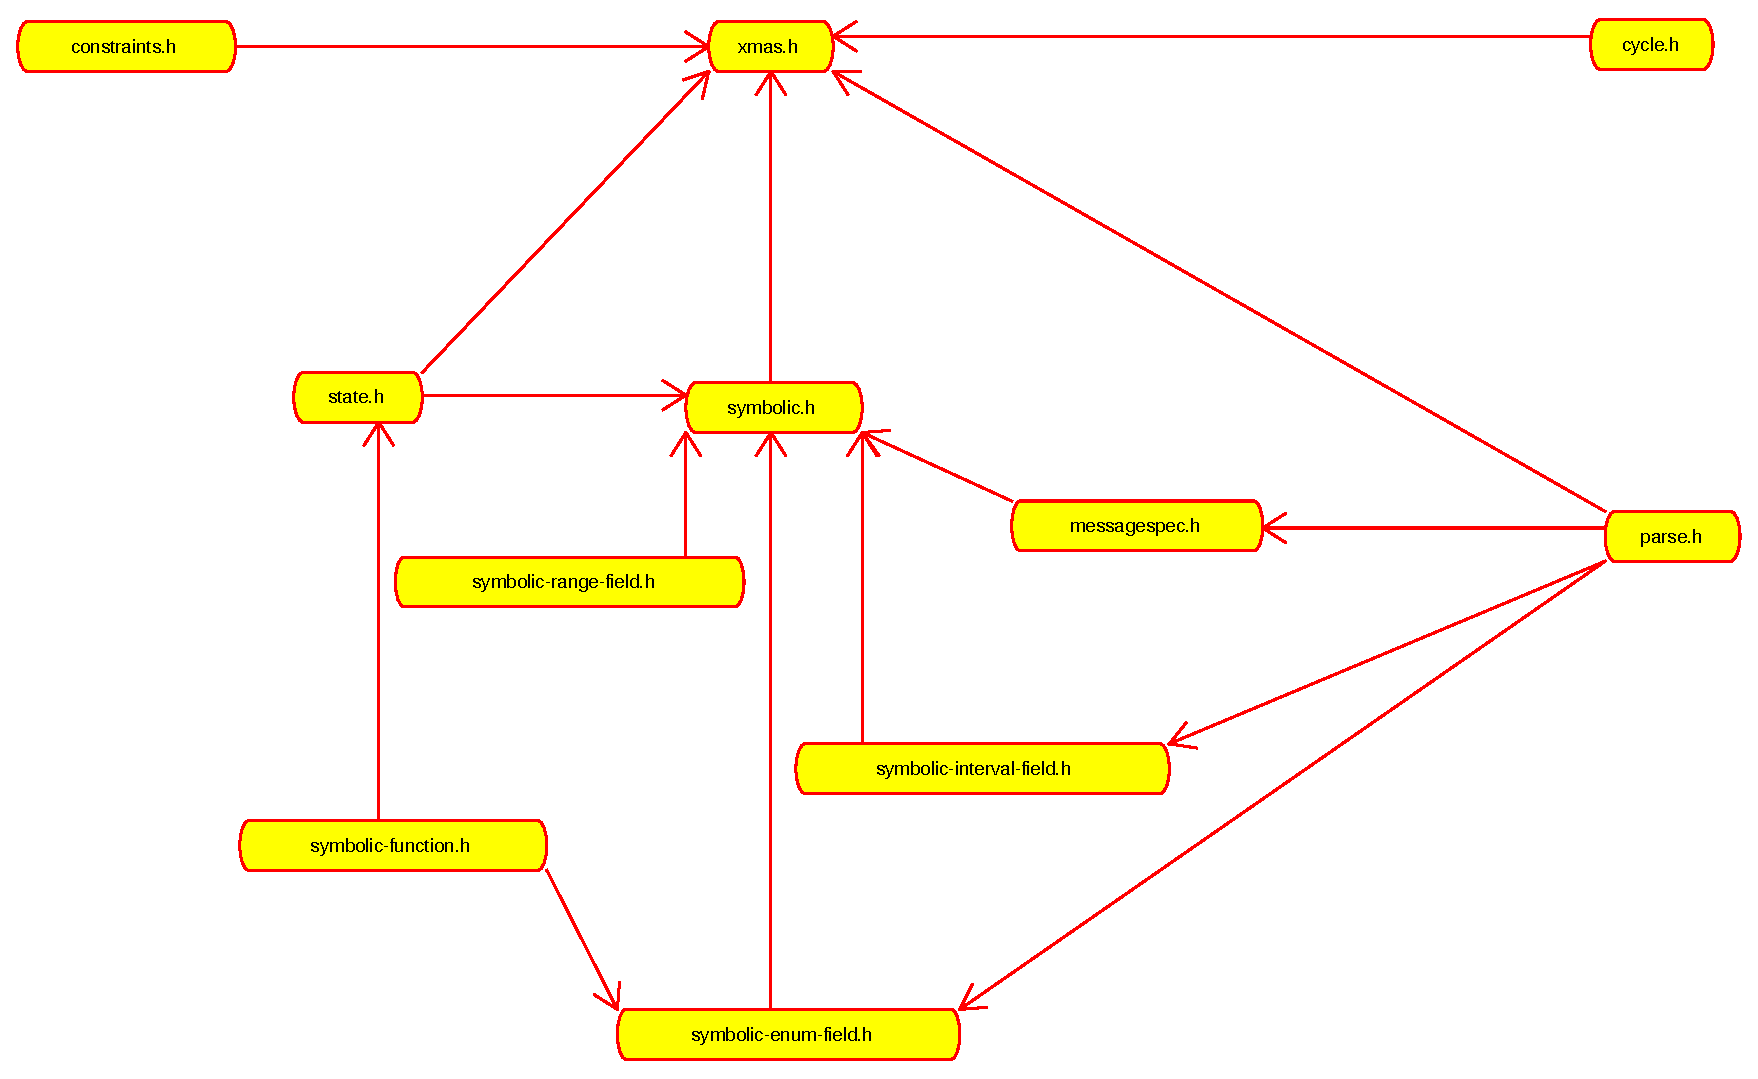
\includegraphics[width=\textwidth]{images/file-dependencies.eps}
  \caption{xMAS header files}
  \label{fig:xmas-headers}
\end{figure}

\end{document}
